%!TEX root = ../main.tex

\section{Copper and Niobium}
\label{sec:metals}

The electrical properties of metals with respect to their temperature has been 
discussed in \autoref{chap:theory}. In the following section, the established theory is compared to the experimentally gathered data from \autoref{sec:setup}.

First and foremost, the high-temperature ($\geq\SI{50}{\kelvin}$) limit of metals is
evaluated. According to \autoref{eq:HT} the resistance should drop off linearly when
the conductor is cooled down. This behaviour is indeed mirrored by both copper and 
niobium. A more precise analysis find the Debye-temperature $\theta$ and the 
Debye-resistance $R_\theta$ as listed in \autoref{tab:fitparams-metal}.

Both sets of measurements do not conform to literature values ($\theta_\text{Cu}
=\SI{343}{\kelvin}$, $\theta_\text{Nb}=\SI{275}{\kelvin}$). This may be caused by
imperfect calibrations of the measured temperature, a bad fitting algorithm or simply
measurement errors. In order to put this disagreement between theory and experiment
into perspective, \autoref{fig:copper} in addition to measurement data shows a 
rough estimate of what one would expect from theory based on a Debye-temperature of 
$\theta = \SI{343}{\kelvin}$.

\begingroup
\renewcommand{\arraystretch}{1.3}
\begin{table}
	\begin{center}
	\caption{Fit parameters for copper and niobium}
	\begin{tabular*}{0.7\textwidth}{@{\extracolsep{\fill}} ccc}
  \toprule
	\hline
  Material & $\theta$ & $R_\theta$  \\
	\hline
  \textbf{Copper} & \SI{266.797\pm1.591}{\kelvin} & \SI{2.011\pm0.027}{\ohm} \\
  \textbf{Niobium} & \SI{224.270\pm4.925}{\kelvin} & \SI{25.137\pm0.661}{\ohm} \\ 
  \bottomrule
	\end{tabular*}
	\label{tab:fitparams-metal}
	\end{center}
\end{table}
\endgroup

In a second part of the analysis, the nonlinear, low-temperature regime is analysed
for both conductors. According to the theory layed out in \autoref{chap:theory}, it 
is expected that the electrical resistance is proportional to $T^5$. To test this 
hypothesis, a polynomial of form $R\propto T^m$ is fitted to the data points found at
the low end of the temperature scale ($<\SI{50}{\kelvin}$). The analysis finds

\begin{align*}
\label{eq:fitparams-slope-metal}
\text{Copper}: m &= 4.834 \pm 0.157 \\
\text{Niobium}: m &= 4.40 \pm 0.71
\end{align*}

While both data sets again do not conform exactly to theory ($m=5$), a clear hint to the $T^5$-behaviour can be extracted from the found results. Lastly, the validity of
\autoref{eq:HT} is evaluated via a combined analysis of both copper and niobium data.
For this porpose the reduced resistivity $\frac{R}{R_\theta}$ is plotted against the
reduced temperature $\frac{T}{\theta}$. This approach should eliminate possible
systematic errors made during the measurement process. A visualisation can be found 
in \autoref{fig:combined-analysis}. A linear regression reveals, that both sets of
data can be described by a line with parameters 

\begin{align*}
% \label{eq:fitparams-combined}
\text{Slope}: m &= 1.185\pm0.006 \\
\text{Intercept}: b &= -0.177\pm0.002, \\ 
\end{align*}

which unsurprisingly resemble the values in \autoref{eq:HT} by a lot. The validity of
the Grüneisen-Borellius formula and underlaying theory is therefore verified.

\begin{figure}
	\centering
	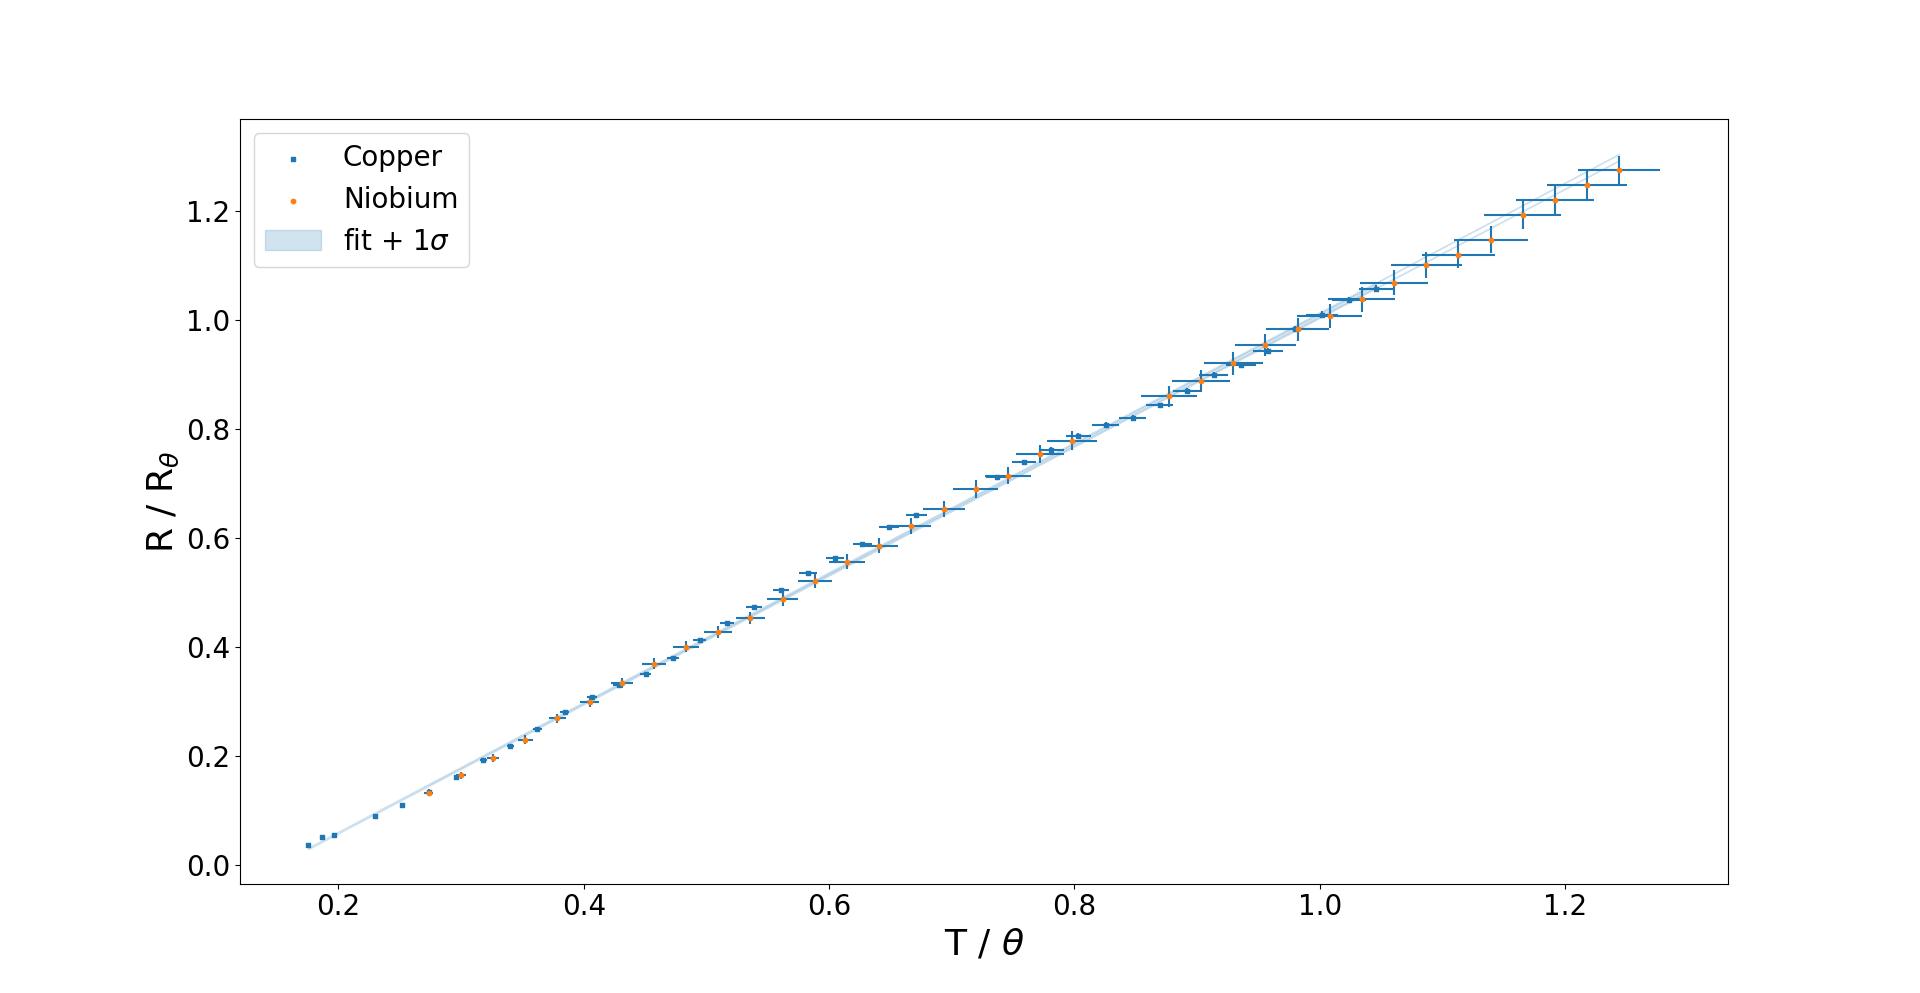
\includegraphics[width=1.0\textwidth]{./fig/combined_analysis.png}
	\caption{Combined analysis of copper and niobium}
	\label{fig:combined-analysis}
\end{figure}


